\section{Progress}

Where are we with design/implementation?

We've implemented moving the goal post for the player to follow, this being implemented on the prior pathfinding demo with the obstacle wall and plain field. The goal post is moved by the player with a drag and drop mechanic, but there's still the question of whether we'll stick with a drag and drop interface for deciding the goal and deciding the start or if we will allow the player to just click on a spot, that will be dependent on how it feels. 


\begin{figure}[htb]
    \centering
    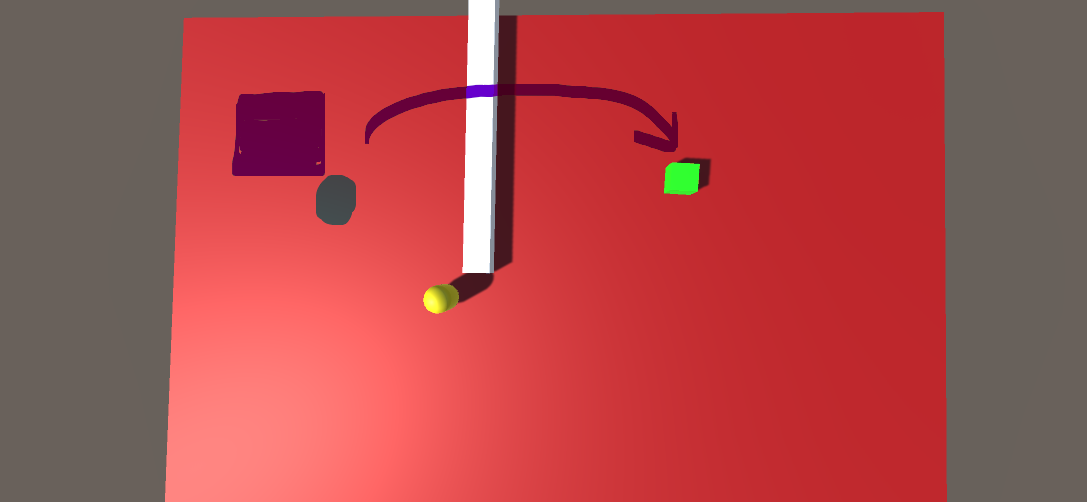
\includegraphics[width=10cm]{../Images/Update3/PathfindingDemo.png}
       \caption{A screenshot of the current pathfinding scene. The blue dot represents where the capsule last stopped to catch the goal at the other side of the wall, then the goal was dragged by the player to the other side where the purple box and arrow point to its new location from where it was dragged from.}
           \label{Fig:Pathfinding Demo 2.0}
  \end{figure}

\begin{flushleft}
We pulled this demo into our car scene now, where the car will now follow a goal to the end of a long straight road. We want to test what path the car will take if given three roads, each with varying difficulty (one road with many turns and curves, one road with one way, and a long curved road.
\end{flushleft}

\begin{figure}[!ht]
    \centering
    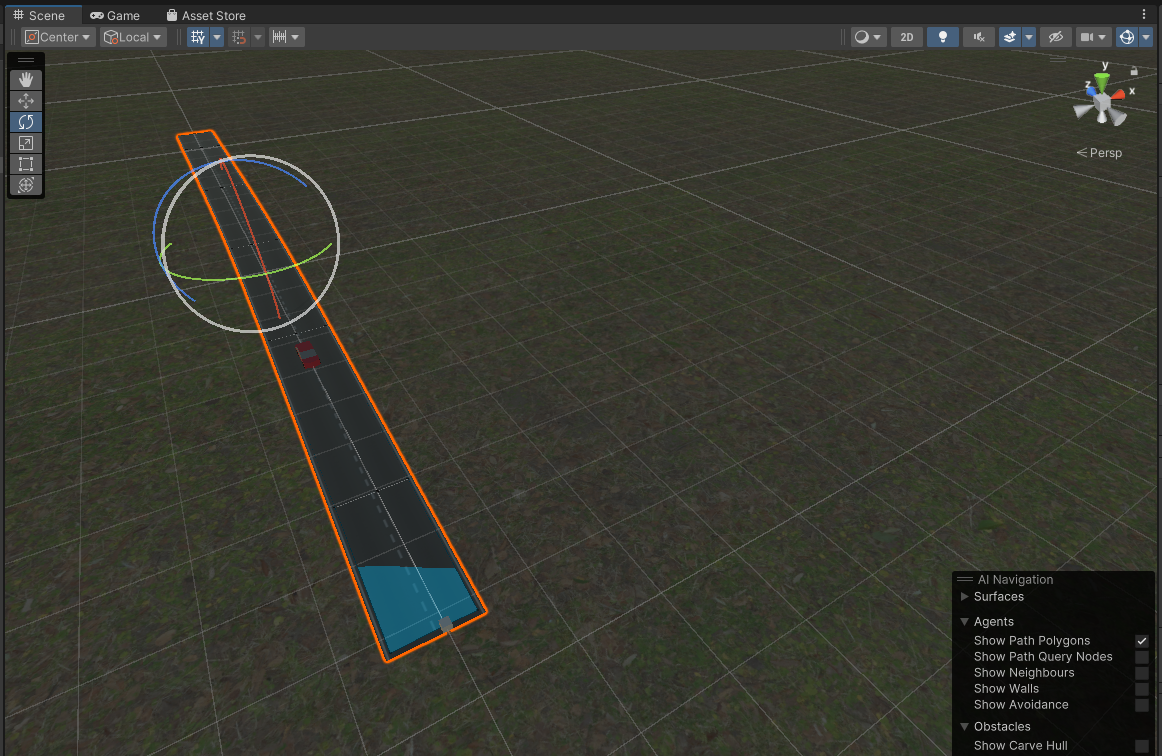
\includegraphics[width=10cm]{../Images/Update3/CarScene.png}
       \caption{The Unity Car Scene with the goal at the end of the road.}
           \label{Fig:UnityCarScene}
   \end{figure}

